\section{Hypothesis Testing and Statistics}
\label{sec:stat_hypo}

This section describes the statistical procedures used in the analyses to be
presented in Chapters~\ref{chap:seach_stop} and \ref{chap:search_hh} that allow
for conclusions to be drawn about the compatibility of the observed data with theories of
BSM physics.
The statistical inference tools described are inherently Frequentist and
are, for the most part, the \textit{de facto} standard for physics analyses searching for evidence of BSM physics
at the large experiments at the LHC.
Their widespread adoption by the experiments at the LHC does not indicate the
philosophical merit of Frequentist inference methodology, but rather highlights the technically simple implementation
of Frequentist hypothesis testing that allows for physics analyses to not get
bogged down in some of the details associated with Bayesian analyses, computational
or otherwise.
Indeed, most people by default think and interact with the world around them
in a Bayesian manner.
Taking the path of least resistance, physicists have tended to opt for the simpler
implementation of reporting their results, which, at the end of the day,
tend to not lose out much in terms of the picture of the objective truth that they draw~\cite{CousinsBayes}.
Section~\ref{sec:hypo_test} will describe, in somewhat general terms, what
hypotheses tests are and the way in which they are performed in ATLAS.
Section~\ref{sec:likelihood} describes the details by which the measurements and systematic
uncertainties of
an analysis are transcribed into the language of the hypothesis test described
in Section~\ref{sec:hypotest} using a likelihood-based test statistic.


%%%%%%%%%%%%%%%%%%%%%%%%%%%%%%%%%%%%%%%%%%%%%%%%%%%%%%%%%%%%%%%%%%%
%%%%%%%%%%%%%%%%%%%%%%%%%%%%%%%%%%%%%%%%%%%%%%%%%%%%%%%%%%%%%%%%%%%
%
% HYPOTHESIS TESTING
%
%%%%%%%%%%%%%%%%%%%%%%%%%%%%%%%%%%%%%%%%%%%%%%%%%%%%%%%%%%%%%%%%%%%
%%%%%%%%%%%%%%%%%%%%%%%%%%%%%%%%%%%%%%%%%%%%%%%%%%%%%%%%%%%%%%%%%%%

\subsection{Hypothesis Testing and the \cls Construction}
\label{sec:hypo_test}

Hypothesis testing starts with the unambiguous formulation of the hypothesis being
tested.
In the search for evidence of BSM physics, there are two hypothesis pitted
against one another.
The first is the \textit{null hypothesis}, denoted $H_0$, which is the hypothesis
subject to the test and corresponds to the SM hypothesis. The null hypothesis is commonly
referred to simply as the background-only (B) hypothesis.
The second hypothesis is the \textit{alternate hypothesis}, denoted $H_1$, and corresponds
to the SM with the addition of the BSM physics process being sought out.
The hypothesis $H_1$ is commonly referred to as the signal-plus-background (S+B) hypothesis.
In both searches presented in Chapters~\ref{chap:search_stop} and \ref{chap:search_hh},
$H_0$ is taken to be the SM.
In the search presented in Chapter~\ref{chap:search_stop}, $H_1$ is taken to be a specific
instantiation of the MSSM ({\color{red}{Section XXX}}), with specific masses of the
stop quark and LSP.
In the search presented in Chapter~\ref{chap:search_hh}, $H_1$ is taken to be the
non-resonant production of Higgs boson pairs.
In this latter case, the $H_1$ hypothesis is indeed a process predicted by the SM ({\color{red}{SECTION XXX about HH pheno and EWSB}}) but
it is one that is not included in the $H_0$ hypothesis.

%%%%%%%%%%%%%%%%%%%%%%%%%%%%%%%%%%%%%%%%%%%%%%%%%%%%%%%%%%%%%%%%%%%
%%%%%%%%%%%%%%%%%%%%%%%%%%%%%%%%%%%%%%%%%%%%%%%%%%%%%%%%%%%%%%%%%%%
%
% TEST STATISTICS
%
%%%%%%%%%%%%%%%%%%%%%%%%%%%%%%%%%%%%%%%%%%%%%%%%%%%%%%%%%%%%%%%%%%%
%%%%%%%%%%%%%%%%%%%%%%%%%%%%%%%%%%%%%%%%%%%%%%%%%%%%%%%%%%%%%%%%%%%
\subsubsection{The Test Statistic and $p$-Values}

In order to perform a hypothesis test in the Frequentist arena, a \textit{test statistic}, $q(x)$,
is defined.
A test statistic is defined using the analysis' measurements $x$ alone and is
used in order to define metrics by which the observed data is said to agree with
one of the two hypothesis, either $H_0$ or $H_1$.
In Section~\ref{sec:likelihood}, the exact form of the likelihood used in modern LHC experiments,
and that used in the analyses discussed in Chapters~\ref{chap:search_stop} and \ref{chap:search_hh},
will be introduced.
Here we will discuss general features of Frequentist test statistics and introduce
some of the language that will be used later on when discussing the results of the
analyses.

The conclusions eventually drawn about a given hypothesis are based on the observed value
of $q(x)$ and where this value lies in relation to the pre-defined \textit{critical region}.
The critical region is defined by a cut value, $q_c$, on the distribution of $q(x)$ under a specified hypothesis.
In the one-sided tests to be considered in the present thesis, $H_1$
will tend to have larger values of $q(x)$ as compared to $H_0$.
The critical region defines two important parameters associated with the hypothesis test.
The first is the quantity $\alpha$, which is referred to as the \textit{significance level},
and is defined as follows,
\begin{align}
    \int\limits_{q_c}^{+\infty} \, f(q | H_0) \, \mathrm{d}q = \alpha,
    \label{eq:sig_level}
\end{align}
where $f(q|H_0)$ is the probability distribution for the test statistic under
the background-only hypothesis.
The quantity $\alpha$ reports the probability for the background-only hypothesis (the SM) to be rejected when it is actually
true. This is commonly referred to as the Type I error rate.
The second quantity is $\beta$ and is defined as,
\begin{align}
    \int\limits_{-\infty}^{q_c} \, f(q|H_1) \, \mathrm{d}q = \beta,
    \label{eq:power_level}
\end{align}
where $f(q|H_1)$ is the probability distribution for the test statistic under
the signal-plus-background hypothesis.
The quantity $\beta$ gives the probability to reject the signal-plus-background hypothesis
when it is actually true. This is commonly referred to as the Type II error rate.
The quantity $(1-\beta)$ is referred to as the \textit{power of the test}.
The better a given physics analysis is at being able to discriminate between the signal
and background, i.e. to have clear separation between the $H_0$ and $H_1$ hypotheses,
the smaller (larger) is $\beta$ (the power of the test).

For simplicity, the two hypotheses $H_0$ and $H_1$ can be generalised by introducing a so-called
`signal strength' parameter, $\mu$, which acts as a multiplicative factor on the signal cross-section
appearing in $H_1$.
The hypothesis $H_0$, then, corresponds to the case $\mu = 0$ and that of $H_1$ corresponds to
$\mu = 1$.
With this general notation, then, the test statistic under either hypothesis is labelled as $q_{\mu}$.

Once a test statistic is specified, and its expected distribution under a given hypothesis is obtained,
$p$-values can be defined in order to compute the probability that the observed data originates from the
considered hypothesis (value of $\mu$).
They are computed as follows,
\begin{align}
    p_{\mu} = \int\limits_{q_{\mu, \text{obs}}}^{+\infty} \, f(q_{\mu} | \mu) \, \mathrm{d}q_{\mu},
    \label{eq:test_stat_pvalue}
\end{align}
where $q_{\mu, \text{obs}}$ is the observed value of the test statistic in data and $f(q_{\mu} | \mu)$ is the probability
density function of $q_{\mu}$ assuming hypothesis $\mu$.
A particular case of Equation~\ref{eq:test_stat_pvalue} is that of $p_0$, which quantifies the agreement of the data with the background-only
hypothesis ($\mu = 0$).
The $p_{\mu}$-value associated with a given hypothesis ($\mu$-value) is typically converted into the equivalent corresponding Gaussian significance, $Z$, defined
as the number of standard deviations that correspond to an upper-tail probability of $p_{\mu}$.
This is illustrated in Figure~\ref{fig:pval_sig}.

As the value of $p_{\mu}$ gets smaller, the confidence that the assumed hypothesis (value of $\mu$) is true
decreases.
At a certain point, it becomes acceptable to say that the assumed hypothesis is incompatible with
reality and the hypothesis described by the particular value of $\mu$ is said to be \textit{excluded}.
In the particle physics community, the conventional threshold to take for the value of $p_{\mu}$
at which point a hypothesis is said to be excluded is $p_{\mu} = 0.05$, corresponding to $Z=1.64$ as
illustrated in Figure~\ref{fig:pval_sig}.
This choice of the $p_{\mu}$-value at which point exclusion is said to occur defines
the critical region, described above, of the test.
The value of $0.05$ corresponds to the significance level of the test (c.f. Equation~\ref{eq:sig_level}), and is referred
to a hypothesis test being performed at the $95\%$ confidence level (CL) (i.e. CL $\equiv (1-\alpha)$)

In order to claim that new physics has been seen, the null hypothesis ($\mu = 0$) must be rejected.
The thresholds at which new physics can be said to have been observed and discovered are
much more stringent than that used for the exclusion of a specified hypothesis.
Incompatibilities with the null-hypothesis at the level of $p_0 = 1.3 \times 10^{-3}$ and
$p_0 = 2.9\times 10^{-7}$ are required in order to state that observation and discovery, respectively,
of new phenomena has occurred.
These thresholds, illustrated in Figure~\ref{fig:pval_sig}, for claiming observation and discovery are the fabled `$3\sigma$' and `$5\sigma$'
$p_0$-value criterion adopted by the particle physics community.

\begin{figure}[!htb]
    \begin{center}
        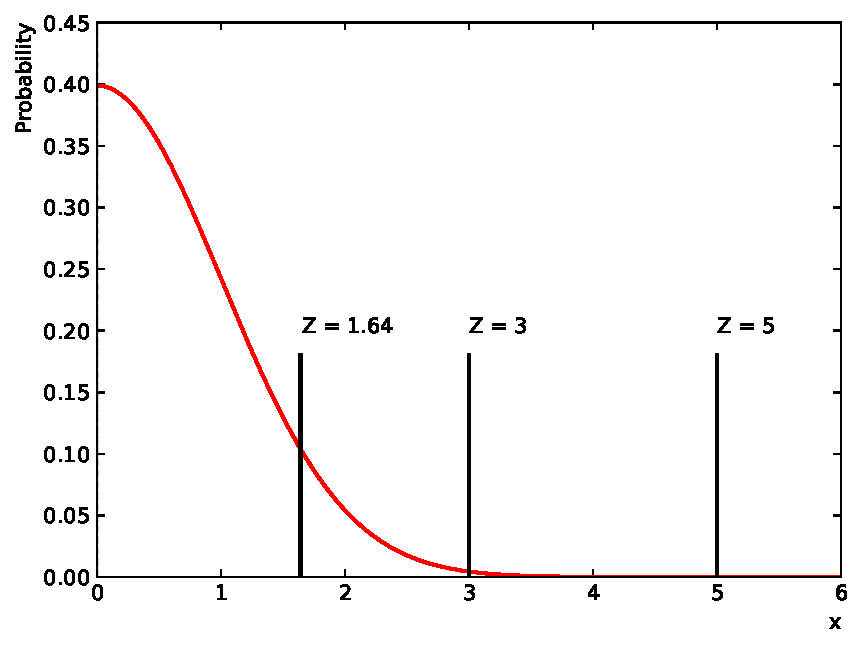
\includegraphics[width=0.48\textwidth]{figures/common_ana/stat_hypo/pval_sig_lin}
        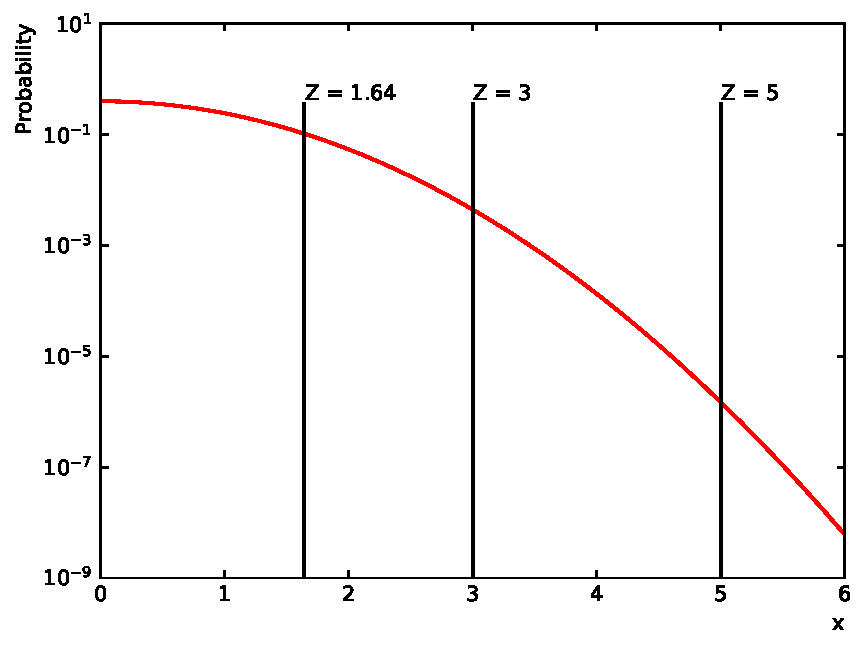
\includegraphics[width=0.48\textwidth]{figures/common_ana/stat_hypo/pval_sig_log}
        \caption{
            Gaussian tail significance levels corresponding to specific $p$-values.
            The significance level of $Z=1.64\sigma$ corresponds to $p = 0.05$,
            that of $Z=3\sigma$ to $p = 1.3 \times 10^{-3}$, and that of
            $Z = 5\sigma$ to $p = 2.9\times 10^{-7}$.
            The area under the tail to the right of each indicated significance level corresponds to
            the associated $p$-value.
            \textbf{\textit{Left}}: Linear $y$-scale. \textbf{\textit{Right}}: Logarithmic $y$-scale.
        }
        \label{fig:pval_sig}
    \end{center}
\end{figure}

%The process of performing a hypothesis test, then, is specified by the following procedure:
%\begin{enumerate}
%    \item Unambiguously define the background-only (the SM prediction) and signal-plus-background (the prediction of the SM with BSM physics added)
%            hypotheses, $H_0$ and $H_1$.
%    \item Define an appropriate test statistic, $t(x)$ (see Section~\ref{sec:likelihood}).
%    \item Construct the distribution of the test statistic under the background-only hypothesis, $g(t|H_0)$.
%    \item Define the desired significance level of the hypothesis, $\alpha$
%    \item Obtain the value of $t(x)$ as observed in data
%    \item If the observed value of $t(x)$ is within the critical region defined by $\alpha$ as in Equation~\ref{eq:sig_level} ($t_{\text{obs}} > t_c$), reject $H_0$.
%            Otherwise, $H_0$ cannot be rejected.
%\end{enumerate}


%%%%%%%%%%%%%%%%%%%%%%%%%%%%%%%%%%%%%%%%%%%%%%%%%%%%%%%%%%%%%%%%%%%
%%%%%%%%%%%%%%%%%%%%%%%%%%%%%%%%%%%%%%%%%%%%%%%%%%%%%%%%%%%%%%%%%%%
%
% THE CLS METHOD
%
%%%%%%%%%%%%%%%%%%%%%%%%%%%%%%%%%%%%%%%%%%%%%%%%%%%%%%%%%%%%%%%%%%%
%%%%%%%%%%%%%%%%%%%%%%%%%%%%%%%%%%%%%%%%%%%%%%%%%%%%%%%%%%%%%%%%%%%

\subsubsection{The \cls Construction}
\label{sec:cls_method}

In searches for new physics, the statement that a given signal hypothesis has been excluded
is an important one.
Once made by the LHC experiments, the specific signal model is essentially considered
no longer important to be searched for.
Therefore, the metrics by which the experiments make claims of exclusion have surrounding them
a wide-ranging literature discussing the merits and drawbacks of the many such metrics
that have been proposed over the years.
The bare $p_{\mu}$-value, for example, extracted from the observed data is subject to statistical fluctuations
and it can lead to unphysical exclusions when a downward fluctuation in the observed
number of events occurs.
This would lead to a premature exclusion of perhaps a broad region of new physics
that would perhaps no longer be looked into by future analyses or experiments.

The standard metric used by the LHC experiments today is known as `\cls'~\cite{CLSReadI,CLSReadII},
and is constructed in such a way as to reduce the likelihood of excluding signal
hypotheses that a search is not a-priori sensitive to.
The \cls metric is given by,
\begin{align}
    \text{CL}_s = \frac{p_{\mu}}{1-p_0},
    \label{eq:cls_def}
\end{align}
where the quantities $p_{\mu}$ and $p_0$ quantify the compatibilities between the data and the signal-plus-background
and background-only hypotheses, respectively.
Downward fluctuations in data, as those described above, will lead to larger values of $p_0$; thus
leading to larger values of \cls that avoid premature exclusion.

At the LHC, the \cls metric is used primarily for performing hypothesis tests aimed at claiming exclusion.
The standard null-hypothesis $p_0$-value is still used for claiming observation and discovery, as described above.
A given signal hypothesis with $\mu = 1$ is considered excluded when $\cls \le 0.05$.
Note that this prescription for exclusion, $\cls \le \alpha$, is generally a stronger requirement than the
standard prescription, $p_{\mu} \le \alpha$.
The \cls metric is also used to compute \textit{upper limits}.
An upper limit on a given signal hypothesis specified by $\mu$
is the largest value of $\mu$ satisfying $\cls \ge 0.05$.
The interpretation being that this corresponds to the largest possible signal cross-section
that is unable to be excluded and therefore smaller values of $\mu$, corresponding
to smaller signal cross-sections, are still consistent with the observed data and cannot therefore
be excluded.
The process of scanning $\mu$ hypotheses and computing the \cls in order to find
an upper limit on $\mu$ is illustrated in Figure~\ref{fig:upper_limit_scan_cartoon}.
%An upper limit on a given signal hypothesis specified by $\mu$ is
%the value of $\mu$ at which $\cls = 0.05$.
%An illustration of how an upper limit is obtained is provided by Figure~\ref{fig:upper_limit_scan_cartoon}.
%%the largest value of $\mu$ describing the signal process that satisfies $\cls \le 0.05$.

\begin{figure}[!htb]
    \begin{center}
        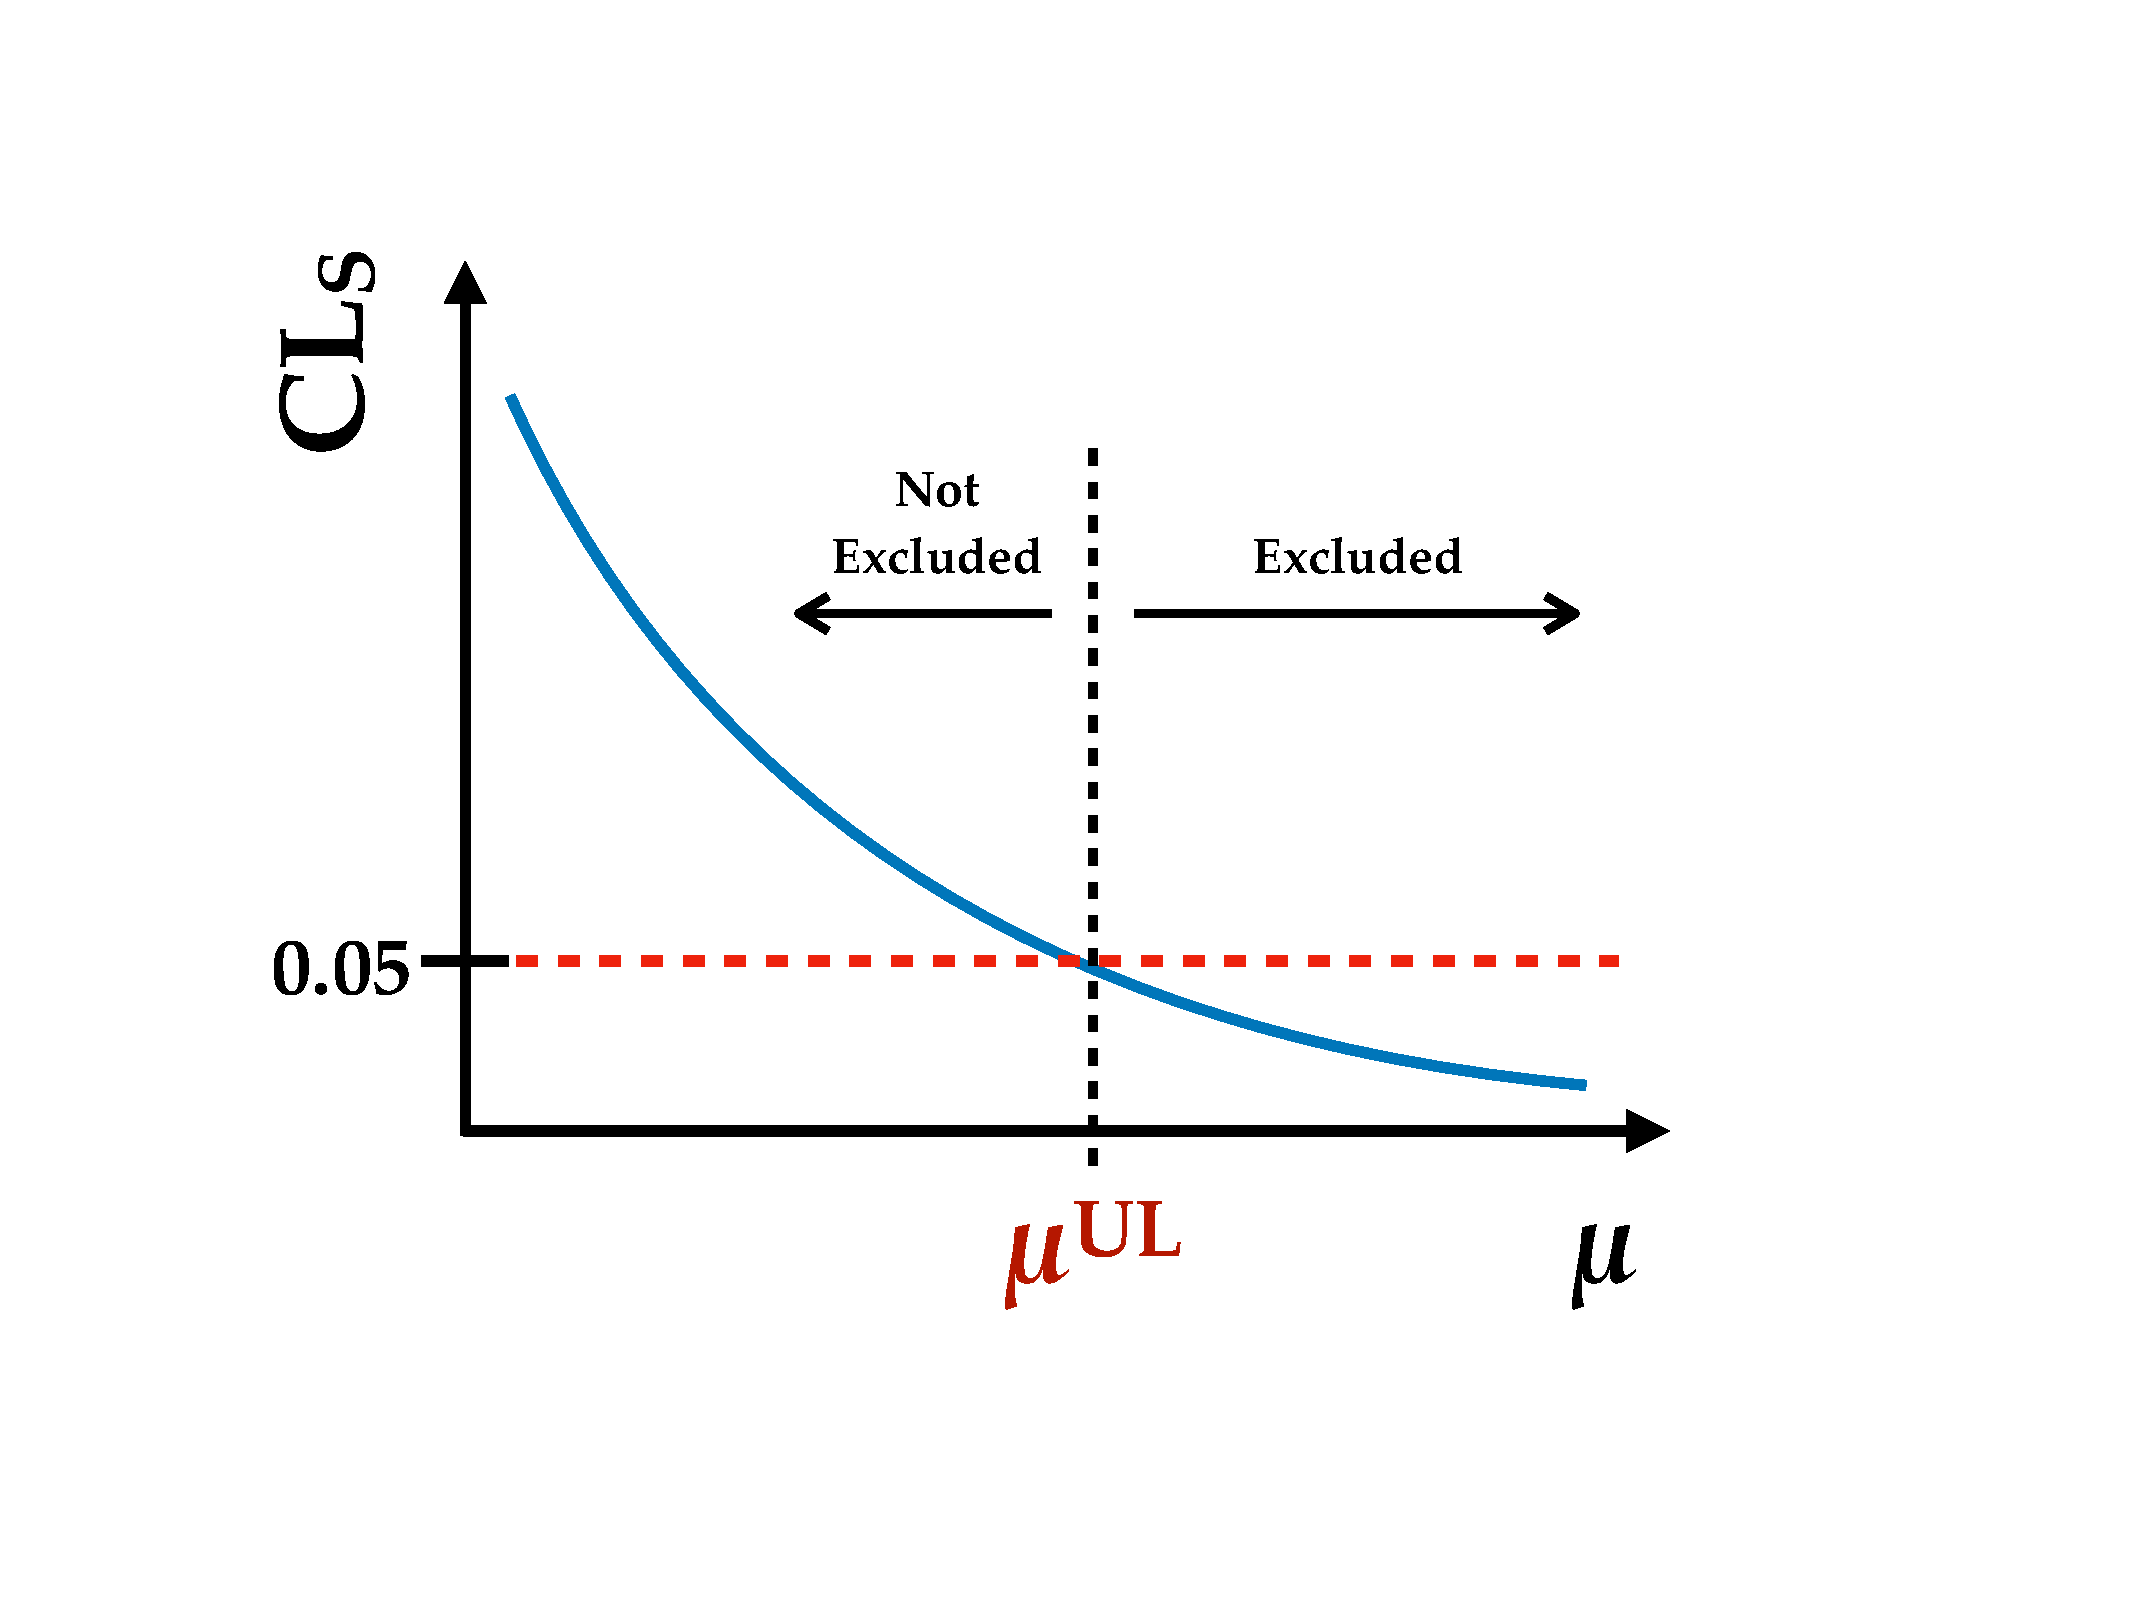
\includegraphics[width=0.5\textwidth]{figures/common_ana/stat_hypo/upper_limit_scan_examplePDF}
        \caption{
            An upper limit scan on the signal strength parameter $\mu$ associated with a signal hypothesis.
            The \cls, given by Equation~\ref{eq:cls_def}, is recomputed for a range of $\mu$ values
            describing a given signal hypothesis.
            This is shown by the blue line.
            The $\mu$ value at which the \cls curve crosses the line $\cls = 0.05$, $\mu^{\text{UL}}$, is the
            upper limit on $\mu$ for the signal hypothesis.
            Values of $\mu$ smaller than $\mu^{\text{UL}}$ remain compatible with the observed data,
            while those values greater than $\mu^{\text{UL}}$ are excluded at $95\%$ CL.
        }
        \label{fig:upper_limit_scan_cartoon}
    \end{center}
\end{figure}

%%%%%%%%%%%%%%%%%%%%%%%%%%%%%%%%%%%%%%%%%%%%%%%%%%%%%%%%%%%%%%%%%%%
%%%%%%%%%%%%%%%%%%%%%%%%%%%%%%%%%%%%%%%%%%%%%%%%%%%%%%%%%%%%%%%%%%%
%
% PROFILE LIKELIHOOD
%
%%%%%%%%%%%%%%%%%%%%%%%%%%%%%%%%%%%%%%%%%%%%%%%%%%%%%%%%%%%%%%%%%%%
%%%%%%%%%%%%%%%%%%%%%%%%%%%%%%%%%%%%%%%%%%%%%%%%%%%%%%%%%%%%%%%%%%%

\subsection{The Profile Likelihood Ratio Test Statistic}
\label{sec:likelihood}

The test statistic associated with many of the LHC experiments, including ATLAS,
and the one used in the analyses to be presented in Chapters~\ref{chap:search_stop} and
\ref{chap:search_hh} is based on a likelihood ratio.
The construction of the test statistic is described in this section.

In the analyses to be presented, so-called `counting experiments' are performed wherein
only the numbers of events, from data and the predicted background and signal,
are used as input.
These numbers are taken from all relevant regions in the analysis: the CRs and the SRs.
The expected number of events populating each region is given by the following:

\begin{align}
    N_r^\text{exp}(\mu_{\text{sig}}, \bm{\mu_{\text{bkg}}}, \bm{\theta}) = \mu_{\text{sig}} \cdot N_{r,\,\text{sig}}^{\text{exp}}(\bm{\theta}) + \sum\limits_{b\,\in \,\text{bkg}} \, \mu_b \cdot N_{r,\,b}^{\text{exp}}(\bm{\theta}),
    \label{eq:test_stat_n_r}
\end{align}
where $\bm{\theta}$ are a set of fit nuisance parameters (NP) associated with the systematic
uncertainties described in Section~\ref{sec:common_systematics},
$\bm{\mu_{\text{bkg}}}$ are normalisation factors associated with the background processes (indexed by `$b$'),
$\mu_{\text{sig}}$ is the signal-strength modifier associated with the signal hypothesis,
$N_{r,\,\text{sig}}^{\text{exp}}$ is the predicted signal yield in region $r$,
and $N_{r,\,b}^{\text{exp}}$ is the predicted background yield in region $r$ for process $b$.
The predicted number of events for each process, signal or background, depend on the $\bm{\theta}$ parameter vector
since systematic variations can adjust the overall normalisation of a given process or adjust
the acceptance of a given process in the phase space probed by the regions indexed by $r$.
Both of these effects result in a change in the predicted rate of a process in a given region.

The observed data yield in each region of the analysis is expected to obey Poisson statistics.
Therefore, the likelihood function $L(\mu_{\text{sig}}, \bm{\mu_{\text{bkg}}}, \bm{\theta})$ is
constructed as a product of Poisson probability terms:
\begin{align}
    L_0(\mu_{\text{sig}}, \bm{\mu_{\text{bkg}}}, \bm{\theta}) = \prod\limits_{r\,\in\,\text{regions}} \, 
            \frac
            {
                \left[N_r^{\text{exp}} ( \mu_{\text{sig}}, \bm{\mu_{\text{bkg}}}, \bm{\theta}) \right] ^ {N_r^{\text{obs}}}
            }
            {
                N_r^{\text{obs}}!
            }
            \cdot
            \exp\left[ N_r^{\text{exp}} ( \mu_{\text{sig}}, \bm{\mu_{\text{bkg}}}, \bm{\theta}) \right],
    \label{eq:likelihood_main}
\end{align}
where $N_r^{\text{obs}}$ is the observed data yield in region $r$.

{\color{red}{REORDER THIS TEXT}} It is standard practice to parametrize the systematic uncertainties associated with the measurements
of the $N_r^{\text{exp}}$ in such a way that $\bm{\theta} = 0$ (all of the $\theta_i$ equal to zero) corresponds to the central (nominal) value
of the set of parameters associated with the uncertainty (e.g. the nominal value of JES).
The values $\theta_i = \pm 1$ represent shifts in the parameter values by their $\pm 1\sigma$
variation, as defined by the systematic uncertainty (e.g. systematic shifts in the value of the JES).
The systematic uncertainties described in Section~\ref{sec:common_systematics} are typically
computed such that, at the level of performing a physics analysis, only the $\pm 1 \sigma$ shifts about the central value
in the associated parameter are known.
Means of interpolation and extrapolation, needed to obtain a smoothly varying response in the
numbers of predicted events as the $\theta$ parameters vary continously between their $\pm 1 \sigma$ values,
are provided by the \textsc{HistFactory} toolkit~\cite{HistFactory}.
The effects of the NP associated with each of the analysis' systematic uncertainties
are implemented as \textit{constraint terms} in the likelihood appearing in Equation~\ref{eq:likelihood_main}.
These terms are typically implemented as Gaussians centered on zero and with a width of 1:
%are implemented as Gaussian \textit{constraint terms}, with wi in the likelihood defined in Equation~\ref{eq:likelihood_main}:
\begin{align}
    L(\mu_{\text{sig}}, \bm{\mu_{\text{bkg}}}, \bm{\theta}) = L_0(\mu_{\text{sig}}, \bm{\mu_{\text{bkg}}}, \bm{\theta})
        \, \cdot \, \prod\limits_{i = 1}^{n} \frac{1}{\sqrt{2 \pi}} \, \exp \left( - \frac{\theta_i^2}{2} \right).
    \label{eq:full_likelihood}
\end{align}
%The constraint terms represent Gaussians centered on 0 and with a width of 1.
%This is equivalent to:
%\begin{align}
%    \theta^{\prime} = \frac{ \theta - \hat{\theta} } {\sigma},
%\end{align}
%allowing for the post-fit NP to be easily compared with the pre-fit ones in the following manner.
%A post-fit value and uncertainty of the NP near 0 and 1, respectively, indicate that the data
The best estimates (maximum likelihood estimates, MLE) for the parameters ($\mu_{\text{sig}}$, $\bm{\mu_{\text{bkg}}}$, $\bm{\theta}$)
are determined in the fit to the observed data, $\bm{N^{\text{obs}}}$, via the maximization
of the likelihood function given by Equation~\ref{eq:full_likelihood}. 
Typically, and equivalently, the negative log likelihood, $-\ln L$, is minimized.
Technically, the minimization of Equation~\ref{eq:full_likelihood} in the analyses to be presented
in Chapters~\ref{chap:search_stop} and \ref{chap:search_hh} is done using \textsc{Miniuit}
via an interface provided by \textsc{RooFit}~\cite{MINUIT,RooFitI}.
The values of all parameters prior to (after) the minimization procedure are referred to as the
`pre-fit' (`post-fit') values.
The pre-fit values for the $\mu_{\text{bkg}}$ parameters are set to 1 and the $\theta_i$ are set to $0$, corresponding
to the central values of the Gaussian-shifted parameters associated with the systematic uncertainties.

The test statistic defined for the analyses to be presented is based on the following
\textit{profile likelihood ratio},
\begin{align}
    \lambda(\mu_{\text{sig}}) \equiv
        \frac{
            L(\mu_{\text{sig}}, \hat{\hat{\bm{\mu}}}_{\text{bkg}}, \hat{\hat{\bm{\theta}}})
        }
        {
            L(\hat{\mu}_{\text{sig}}, \hat{\bm{\mu}}_{\text{bkg}}, \hat{\bm{\theta}})
        },
    \label{eq:likelihood_ratio}
\end{align}
where in the numerator the parameters $(\bm{\mu}_{\text{bkg}}, \bm{\theta})$ are fit to their MLE values
for a given value of the assumed value of the signal-strength parameter $\mu_{\text{sig}}$.
In the denominator, the full set of parameters ($\mu_{\text{sig}}$, $\bm{\mu_{\text{bkg}}}$, $\bm{\theta}$) are
equal to their MLE values.
The likelihood ratio defined in Equation~\ref{eq:likelihood_ratio} is used to define the
final test statistic relevant to the analyses,
\begin{align}
    q_{\mu_{\text{sig}}} = - 2 \ln \lambda (\mu_{\text{sig}}),
    \label{eq:pll_test_stat}
\end{align}
which is used to perform the hypothesis tests described in Section~\ref{sec:hypo_test}.

\subsubsection{Profile Likelihood Fit Determination of Background Constraints}

We note here that the quantites described by $\bm{\mu_{\text{bkg}}}$ in Equations~\ref{eq:test_stat_n_r}--\ref{eq:pll_test_stat} correspond to normalisation correction
factors for a given SM background process.
In the analyses to be presented in Chapters~\ref{chap:search_stop} and \ref{chap:search_hh},
for the background processes for which a dedicated CR is not defined, the associated $\mu_b$ are
set to 1 and are not allowed to vary during the fit (i.e. their pre-fit and post-fit values are equal).
%these values are set to one for all background processes that do not have a dedicated
%CR and are not allowed to vary from this value during the fit procedure.
For those processes for which a dedicated CR is defined, the associated $\mu_b$ parameters
are analogous to the normalisation correction factors described in Section~\ref{sec:control_region_method} and
are unconstrained in the fit procedure.
They are therefore said to `freely float' during the fit and 
their post-fit value does not necessarily correspond to their pre-fit one.
Given the low numbers of events typically expected in the SRs, and the relatively
large numbers and purities expected in the CRs, the post-fit values of the $\mu_b$ typically
correspond to those values expected from the simple computations provided by Equation~\ref{eq:mu_fac}
and/or Equation~\ref{eq:mu_fac_expand}.
An additional note is that in the signal-plus-background hypotheses with $\mu_{\text{sig}} \ne 0$, if
the CRs have a non-negligible contamination of signal events, however, this correspondence will generally not be true
since the post-fit values of the $\mu_b$ will depend on a given value of the $\mu_{\text{sig}}$ parameter.
The desire to construct a robust background-only model is one of the motivating factors, then,
in designing analyses in such a way as to minimize the signal contamination in the CRs.

\subsubsection{Profiling}
\label{sec:profiling}

The Gaussian constraint terms in Equation~\ref{eq:full_likelihood}, centered on 0 and with widths of 1,
are equivalent to transforming the $\bm{\theta}$ parameters associated with the systematic uncertainties as follows,
\begin{align}
    \bm{\theta}^{\prime} = \frac{\bm{\theta} - \bm{\hat{\theta}}}{\bm{\hat{\sigma}}},
    \label{eq:theta_gaus}
\end{align}
where the quantity $\bm{\sigma}$ corresponds to the initial widths of the $\pm 1 \sigma$ variations
associated with the systematic variation represented by $\bm{\theta}$.
Equation~\ref{eq:theta_gaus} normalises all NP to facilitate the easy comparison of their pre- and post-fit values and uncertainties.
For a given NP, then, a post-fit value and uncertainty near 0 and 1, respectively, indicate
that the data was not able to adjust the NP.
Changes in the post-fit NP values (uncertainties) are referred to as NP `pulling' (`profiling').
NP values may be pulled far from zero in order to maximize the overall agreement of the background prediction
with data during the fit procedure.
NP may be profiled in such a way that the post-fit uncertainties on the NP are smaller than the
the initial estimate of the uncertainty provided by auxiliary measurements and data.
Such a case indicates that the initial prior on the impact of the systematic uncertainty was too
large and that the uncertainties may be reduced so as to be more compatible  with the range allowed by
the data statistics relevant for the analysis at hand.
This potential for the profiling mechanism to reduce the overall impact of systematic uncertainties
on an analysis' results is seen as a general benefit of the profile likelihood prescription described
by Equations~\ref{eq:likelihood_ratio} and \ref{eq:pll_test_stat}.
The interpretation of this is that the profiling mechanism allows for the impact of the systematic uncertainties
to be more accurately characterised in the phase space in which they are being applied, as opposed
to that of the auxiliary measurements in which they are initially derived.

\subsubsection{Profiling Example 1}
\label{sec:profiling_example_1}

{\color{red}{Not sure if I want this}}

\subsection{Asymptotic Formulation of Likelihood Ratio Tests}

{\color{red}{Describe the asympotitc formula used for the analysis to be presented and illustrate
examples of how various p values are obtained, as well as how analysis sensitivity is optimized}}
